\documentclass[twoside]{article}
\usepackage[a4paper]{geometry}
\geometry{verbose,tmargin=2.5cm,bmargin=2cm,lmargin=2cm,rmargin=2cm}
\usepackage{fancyhdr}
\pagestyle{fancy}

% nastavení pisma a~češtiny
\usepackage{lmodern}
\usepackage[T1]{fontenc}
\usepackage[utf8]{inputenc}
\usepackage[czech]{babel}

% odkazy
\usepackage{url}

\usepackage{float}
% vícesloupcové tabulky
\usepackage{multirow}
\usepackage{amssymb}
\usepackage{gensymb}
\usepackage{bbold}
\usepackage{mathtools}
\usepackage{commath}

% vnořené popisky obrázků
\usepackage{subcaption}

% automatická konverze EPS 
\usepackage{graphicx} 
\usepackage{epstopdf}
\usepackage{amsmath}
\epstopdfsetup{update}

% odkazy a~záložky
\usepackage[unicode=true, bookmarks=true,bookmarksnumbered=true,
bookmarksopen=false, breaklinks=false,pdfborder={0 0 0},
pdfpagemode=UseNone,backref=false,colorlinks=true] {hyperref}

% Poznámky při překladu
\usepackage{xkeyval}	% Inline todonotes
\usepackage[textsize = footnotesize]{todonotes}
\presetkeys{todonotes}{inline}{}
\graphicspath{{./images}}

%https://tex.stackexchange.com/questions/2783/bold-calligraphic-typeface
\DeclareMathAlphabet\mathbfcal{OMS}{cmsy}{b}{n}

% Zacni sekci slovem ukol
\renewcommand{\thesection}{Úkol \arabic{section}}
% enumerate zacina s pismenem
\renewcommand{\theenumi}{\alph{enumi}}

% smaz aktualni page layout
\fancyhf{}
% zahlavi
\usepackage{titling}
\fancyhf[HC]{\thetitle}
\fancyhf[HLE,HRO]{\theauthor}
\fancyhf[HRE,HLO]{9. prosince 2021}
 %zapati
\fancyhf[FLE,FRO]{\thepage}

% údaje o autorovi
\title{Robotika - Kalibrace paralelního manipulátoru}
\author{Vojtěch Michal}
\date{9. prosince 2021}

\begin{document}

\maketitle

\section{Kalibrované parametry}

Cílem kalibrace manipulátoru je zpřesnit devět číselných parametrů umístěných do vektoru
\begin{equation}
	\vec{d}^T = \begin{bmatrix}
		l_{21} & l_{22} & l_{12} & \gamma_1 & \gamma_2 & P_{1x} & P_{1y} & P_{2x} & P_{2y}
	\end{bmatrix}.
\end{equation}
Jedná se po řadě o délky ramen (parametry $l_{ij}$), sklon pohybu posuvného kloubu ($\gamma_1$), offset nuly rotačního kloubu ($\gamma_2$)
a souřadnice bodů $P_{1,2}$, kde je robot poután k rámu. Význam parametrů je i z nákresu na obrázku \ref{fig:nakres}.
Nepřesné počáteční odhady těchto parametrů funkce \textit{mycalib} obdrží v rámci parametrů od volajícího kódu. Zpřesněné hodnoty jsou uloženy
v její návratové hodnotě.

\section{Kalibrační body}
Pro maximálně rovnoměrnou kalibraci ve všech rozumných bodech pracovního prostoru byly kloubové souřadnice vybírány následujícícm způsobem.
Pracovní prostor se pokryl rovnoměrně rozmístěnými body (kartézský součin vektoru \textit{-100:$n$:100} se sebou).
Následně byla pro všechny body vypočtena analyticky IKT pro stanovení, zda je daný bod manipulátorem dosažitelný či nikoli.
Hodnota $n$ byla zvolena tak, aby bylo z IKT vyšlo méně než 250 dosažitelných bodů.
Na $n = 1.45$ připadalo 249 unikátních dosažitelných kalibračních bodů rozmístěných po pracovním prostoru,
jejich polohy jsou vykresleny na obrázku \ref{fig:kalib_body}.

\begin{figure}[htbp]
	\centering
	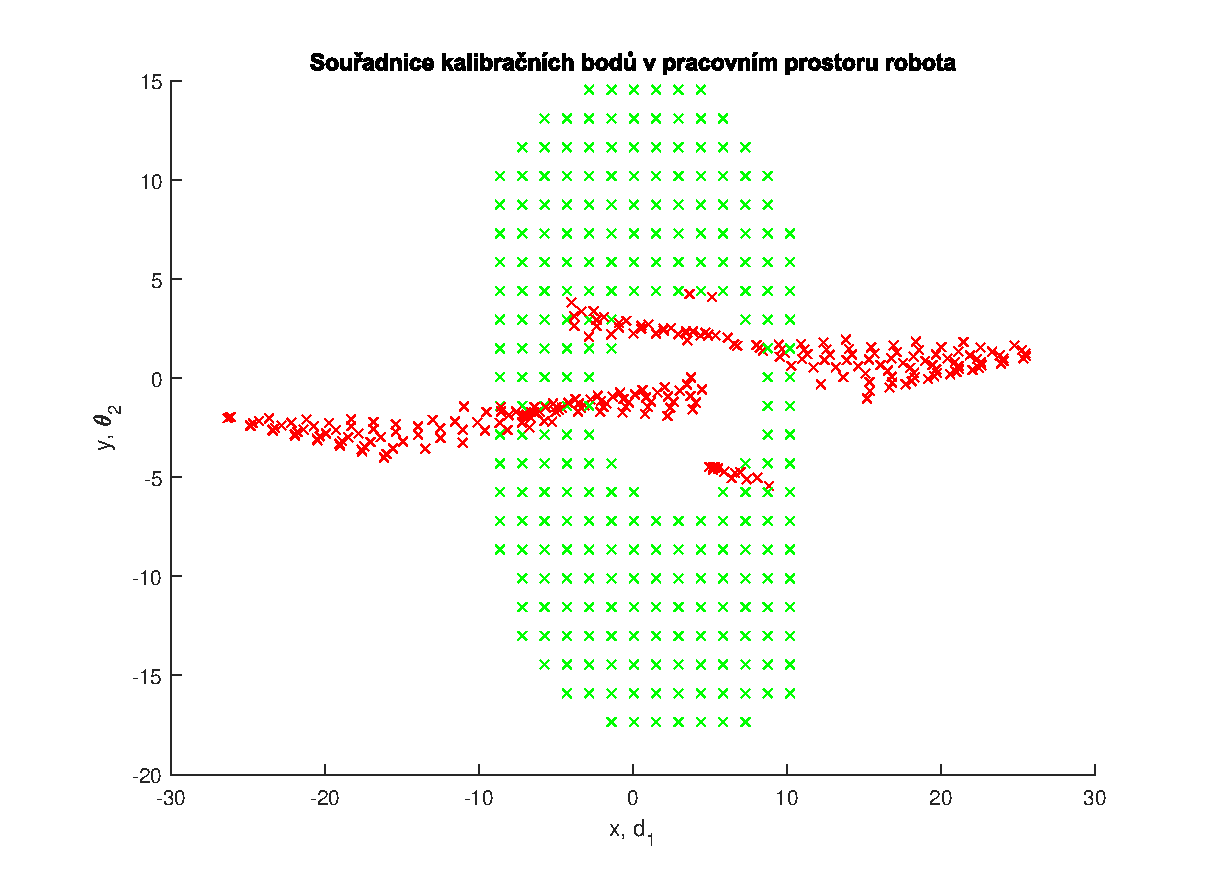
\includegraphics[width=0.7\linewidth]{kalib_body.eps}
	\caption{Zvolené kalibrační body. Červeně kloubové souřadnice $d_1$, $\theta_2$, zeleně polohy chapadla $x$, $y$.}
	\label{fig:kalib_body}	
\end{figure}

\section{Konvergence numerické metody}

Na \ref{fig:presnost} jsou vykresleny průběhy věličin relevantních pro ohodnocení kvality kalibrace.
Graf \ref{fig:chyba} ukazuje vývoj euklidovské normy chybového vektoru v závislosti na počtu provedených iterací numerického optimalizačního algoritmu.
Je patrné, že již po druhé iteraci se algoritmus ustálil na lokálním minimu chybové funkce a další iterace nebyly potřebné.
Totéž dokládá obrázek \ref{fig:delta_d}, na kterém je vykreslen vývoj euklidovské normy vektoru $\Delta d$ použitém v aktualizačním kroku $k$-té iterace $\vec{d}_{k+1} = \vec{d}_{k} + \Delta \vec{d}$.
Použitý optimalizační algoritmus je \textbf{Gauss-Newtonova iterační metoda}.

\begin{figure}[htbp]
	\centering
	\begin{subfigure}{0.45\linewidth}
		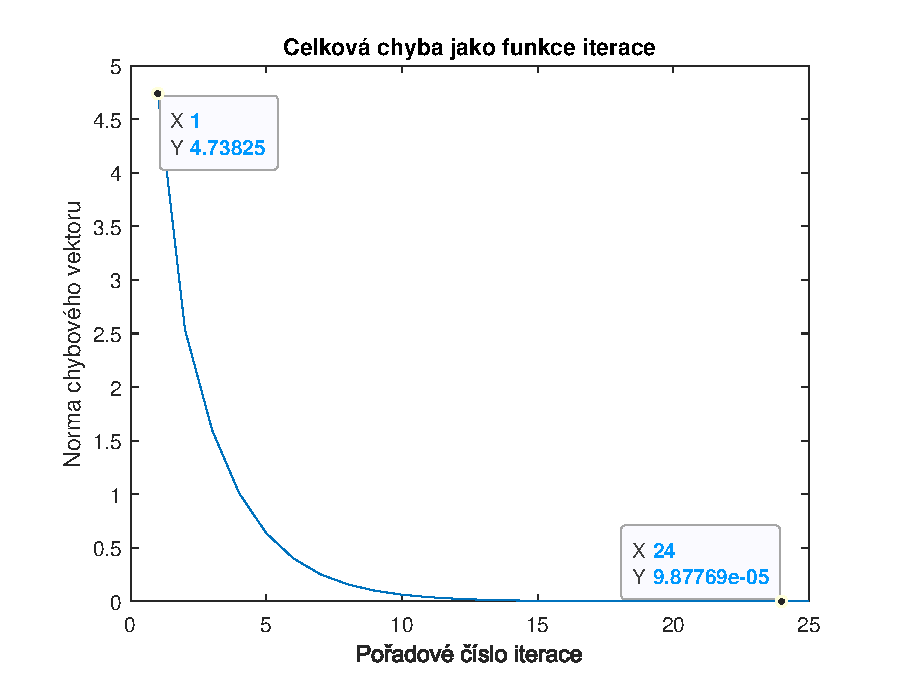
\includegraphics[width=\linewidth]{chyba.eps}
		\caption{Ustalování normy odchylek chyb během kalibrace}
		\label{fig:chyba}
	\end{subfigure}
	\begin{subfigure}{0.45\linewidth}
		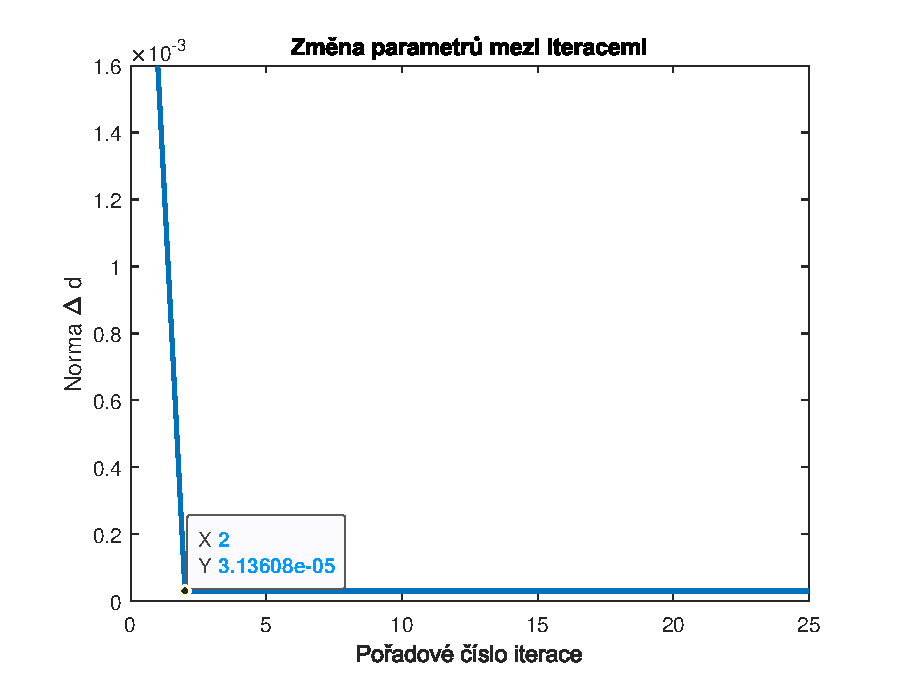
\includegraphics[width=\linewidth]{delta_d.eps}
		\caption{Ustalování $\lVert \Delta \vec{d} \lVert$ během kalibrace}
		\label{fig:delta_d}
	\end{subfigure}
	\caption{Vývoj velikosti vektorů odchylek a aktualizací parametrů v průběhu kalibrace}
	\label{fig:presnost}
\end{figure}

\section{Nákres}

Na obárzku \ref{fig:nakres} jsou rukou psané poznámky k úloze a náčrtek s významem jednotlivých proměnných.

\begin{figure}[htbp]
	\centering
	\includegraphics[width=\linewidth]{nakres.jpg}
	\caption{Nákres úlohy a ručně psané poznámky}
	\label{fig:nakres}	
\end{figure}

\end{document}


